\section{Implementación del prototipo}\label{section:prototype}

El prototipo implementado se compone de cuatro componentes: Crawler, Cat\'alogo de Datos, Generador de Consultas 
e Interfaz de Usuario; los cuales se corresponden al diseño de sistema propuesto en el cap\'itulo \ref{chapter:proposal}. 
La l\'ogica de los an\'alisis sintáctico y l\'exico del DSL propuesto fue incluida dentro del Generador de Consultas. 
Por cuestiones de tiempo no se pudo concretar una implementaci\'on del Generador de Pipelines.

\subsection{Organización de los archivos}

La l\'ogica de cada uno de los componentes de la aplicaci\'on se encuentra separada por carpetas. Cada componente 
posee su propia carpeta identificada con el nombre del componente en ingl\'es, a excepción de la Interfaz de Usuario 
cuya carpeta es nombrada \textbf{pages} y su script principal se encuentra en la ra\'iz del proyecto con el nombre de 
\textbf{MainPage.py}. Todos los datos derivados de la ejecución de la l\'ogica de cada uno de los componentes 
se almacena dentro de la carpeta \textbf{data}. La carpeta \textbf{utils} guarda scripts de algoritmos usados 
en varias partes de la aplicaci\'on, concretamente posee scripts con algoritmos para la carga y escritura de los 
grafos y \'arboles de join en el disco.

\subsection{Fuentes de datos}

El prototipo solo es capaz de manejar una sola fuente de datos a la vez, aunque si se pueden considerar varias 
fuentes de datos para un mismo almac\'en de datos de destino. Para esto se debe definir un script del DSL por 
cada fuente de datos que alimente el almac\'en de datos. Las primeras consultas de creación generadas que se ejecuten 
para dicho almac\'en de datos van a determinar el nombre de las dimensiones y tablas de hechos, as\'i como 
como el nombre de sus atributos, sus tipos y restricciones. Luego, para alimentar el almac\'en de datos con otras 
fuentes basta con ejecutar solamente las consultas de selecci\'on generadas a partir del script correspondiente a 
dicha fuente y luego insertar en el almac\'en los valores extra\'idos.

\subsection{Crawler}

El Crawler constituye un elemento de interdependencia dentro del prototipo en relación con los sistemas 
de gestión de bases de datos, específicamente con los SGBD de las fuentes de datos. Con el objetivo de lograr una 
mayor extensibilidad, se plantea la creación de una clase abstracta llamada \textbf{crawler}, la cual establecerá 
el comportamiento general de este componente. De este modo, se delega a las implementaciones específicas para cada 
SGBD la definición de la forma en que se llevan a cabo las operaciones, como se muestra en la figura \ref{fig:crawler}.
A continuación de se muestra la definición de la clase crawler.

\begin{lstlisting}[label={code:crawler}, caption={clase abstracta crawler}, language={python}]
    import abc

    class Crawler(metaclass=abc.ABCMeta):
        def __init__(self, dbname, user, password, host, port) -> None:
            self.dbname = dbname
            self.user = user
            self.password = password
            self.host = host
            self.port = port
            self._db_params = {'dbname': dbname, 'user': user, 'password': password, 'host': host, 'port': port}
            self._metadata_str = ''
            self._db_dict = {}

        @abc.abstractmethod
        def explore_db(self):
            pass
        
        @abc.abstractmethod
        def export_metadata_to_file(self):
            pass

\end{lstlisting}

La definición de esta clase se encuentra en el archivo \textbf{crawler.py} de la carpeta del componente. Los 
campos de la clase se corresponden con la informaci\'on necesaria para establecer una conexi\'on con una base de 
datos. 

El m\'etodo \textbf{explore\_db} se encarga de recopilar los metadatos mencionados en el cap\'itulo \ref{chapter:proposal}
y almacenarlos en el diccionario \textbf{\_db\_dict} el cual tiene como llaves los nombres de las tablas de la base 
de datos y como valores otros diccionarios que poseen dos llaves: \textbf{attributes} y \textbf{relations}. 
El valor de \textbf{attributes} es una lista de tuplas de dos o tres elementos, una por cada atributo de la tabla. 
Las tuplas de dos elementos almacenan el nombre del atributo y el tipo, las de tres almacenan adem\'as un indicador 
que expresa si el atributo es llave primaria, for\'anea o ambas. El valor de \textbf{relations} es una lista de 
tuplas de tres elementos, una por cada atributo llave for\'anea de la tabla. El primer elemento es el nombre 
de la llave for\'anea en la tabla, el segundo el nombre de la tabla referenciada y el tercero el atributo referenciado. 
Adem\'as, el m\'etodo \textbf{explore\_db} tiene la responsabilidad de llenar la cadena de texto \textbf{\_metadata\_str} 
que almacena los metadatos recopilados en un formato m\'as expresivo para luego ser mostrado al usuario.

El m\'etodo \textbf{export\_metadata\_to\_file} se encarga guardar \textbf{\_db\_dict} y \textbf{\_metadata\_str} en el disco, 
en la ruta \textbf{data/schemas}. La carpeta \textbf{schemas} contiene una carpeta por cada base de datos identificada 
por el nombre de dicha base de datos en la cual se almacena en formato json \textbf{\_db\_dict} y en formato txt 
\textbf{\_metadata\_str}.

En esta primera entrega del prototipo solo se le di\'o implementaci\'on a un crawler para PostgreSQL. Su l\'ogica 
se encuentra en el archivo \textbf{postgreSQL\_crawler.py}. Los metadatos son recopilados mediante consultas realizadas
a la tabla \textbf{information\_schema} de base de datos fuente ejecutadas 
utilizando el adaptador de PostgreSQL para python \textbf{psycopg2}.

\begin{figure}[htb]
    \centering
    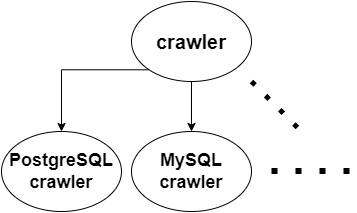
\includegraphics[width=0.5\textwidth]{Graphics/crawler_class.drawio.png}
    \caption{Jerarqu\'ia de la clase abstracta crawler}
    \label{fig:crawler}
\end{figure}


\subsection{Cat\'alogo de Datos}

El Cat\'alogo de Datos es un servido de base de datos de Neo4j. La idea es que exista un base de datos Neo4j por cada 
fuente de datos, sin embargo la versi\'on community de Neo4j utilizada solo permite la creación de una sola base de datos. 
Por tanto, cada vez que se establece conexi\'on con otra base de datos fuente la informaci\'on existente en cat\'alogo es 
sobreescrita. Esto no supone un problema para la inferencia de Joins puesto que el grafo de join obtenido a partir 
del Cat\'alogo de Datos es almacenado en el disco y recuperado cuando es necesario su uso. Para versiones m\'as avanzadas 
del prototipo hay que considerar la utilizaci\'on de Neo4j Enterprise.

La comunicaci\'on de la aplicaci\'on con el Cat\'alogo de Datos es mediada por la clase \textbf{DataCatalogHandler} 
presente en el script \textbf{handler.py} de la carpeta \textbf{data\_catalog}. A continuación se muestra parte 
del c\'odigo de dicha clase.

\begin{lstlisting}[label={code:catalog}, caption={Clase DataCatalogHandler}, language={python}]
    class DataCatalogHandler():
        def __init__(self, db_dict, db_name, user, password, uri) -> None:
            self.db_dict = db_dict
            self._user = user
            self._password = password
            self._uri = uri
            self.db_name = db_name
            self.join_graph = None

        def create_graph_database(self):
            # Omitted implementation

        def export_join_graph(self):
            # Omitted implementation

\end{lstlisting}

El campo \textbf{db\_dict} es el diccionario de la base de datos confeccionado por el Crawler, \textbf{db\_name} es 
nombre de la base de datos fuente, \textbf{join\_graph} almacena el grafo de join derivado y el resto de atributos 
son los necesarios para establecer una conexi\'on con una base de datos de Neo4j, especificada por el campo \textbf{\_uri}. 

El m\'etodo \textbf{create\_graph\_database} crea en la base de datos especificada un nodo por cada llave (tabla) 
en \textbf{db\_dict} con las propiedades \textbf{name} que almacena el nombre de la tabla, \textbf{attributes} que 
es la lista aplanada de tuplas correspondiente a la llave attributes del diccionario que contiene \textbf{db\_dict} 
indexado en el nombre de la tabla en cuesti\'on y \textbf{pks} que es una lista con los nombres de los atributos que 
son llaves primarias. Adem\'as, se crea una relación por cada  